% Created by tikzDevice version 0.10.1 on 2016-02-27 12:54:11
% !TEX encoding = UTF-8 Unicode
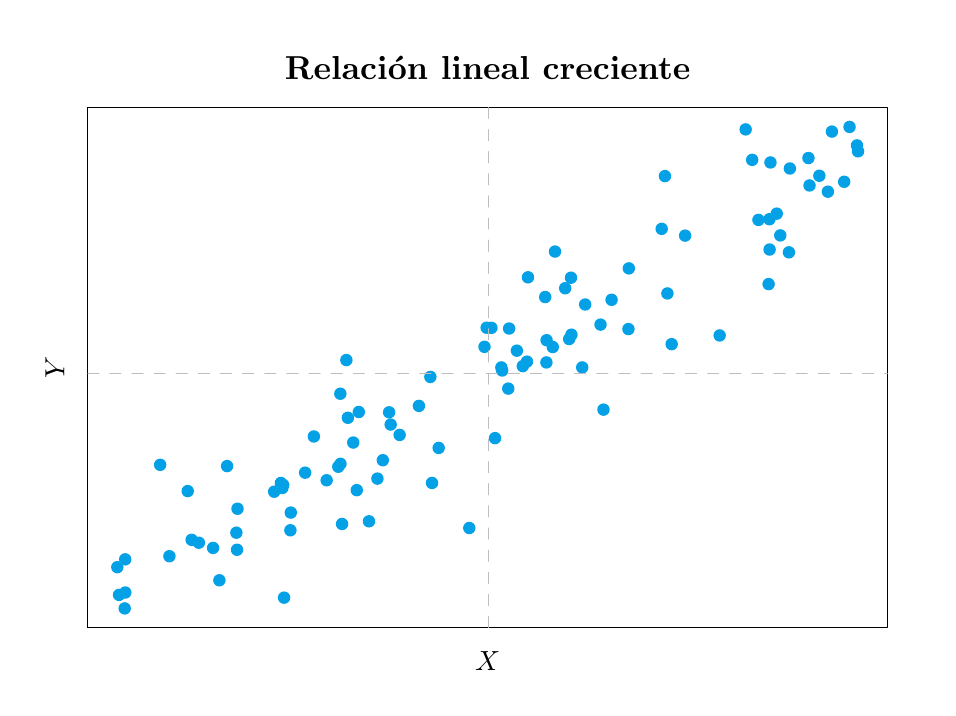
\begin{tikzpicture}[x=1pt,y=1pt]
\definecolor{fillColor}{RGB}{255,255,255}
\path[use as bounding box,fill=fillColor,fill opacity=0.00] (0,0) rectangle (325.21,238.49);
\begin{scope}
\path[clip] ( 21.68, 21.68) rectangle (310.76,209.58);
\definecolor{fillColor}{RGB}{5,161,230}

\path[fill=fillColor] (267.74,145.83) circle (  2.25);

\path[fill=fillColor] (229.09,165.79) circle (  2.25);

\path[fill=fillColor] (112.98,106.21) circle (  2.25);

\path[fill=fillColor] (264.06,169.03) circle (  2.25);

\path[fill=fillColor] (167.57,130.03) circle (  2.25);

\path[fill=fillColor] ( 92.65, 32.53) circle (  2.25);

\path[fill=fillColor] ( 47.87, 80.52) circle (  2.25);

\path[fill=fillColor] ( 33.02, 33.52) circle (  2.25);

\path[fill=fillColor] (187.00,141.15) circle (  2.25);

\path[fill=fillColor] (194.23,144.34) circle (  2.25);

\path[fill=fillColor] ( 95.08, 63.27) circle (  2.25);

\path[fill=fillColor] ( 69.27, 38.81) circle (  2.25);

\path[fill=fillColor] (250.05,127.27) circle (  2.25);

\path[fill=fillColor] (141.38,101.82) circle (  2.25);

\path[fill=fillColor] (189.74,123.09) circle (  2.25);

\path[fill=fillColor] (126.38, 75.54) circle (  2.25);

\path[fill=fillColor] ( 75.82, 64.65) circle (  2.25);

\path[fill=fillColor] (128.33, 82.19) circle (  2.25);

\path[fill=fillColor] (196.33,148.14) circle (  2.25);

\path[fill=fillColor] (100.26, 77.69) circle (  2.25);

\path[fill=fillColor] (282.52,181.47) circle (  2.25);

\path[fill=fillColor] (180.42,117.81) circle (  2.25);

\path[fill=fillColor] ( 75.65, 49.84) circle (  2.25);

\path[fill=fillColor] (113.03, 80.89) circle (  2.25);

\path[fill=fillColor] (275.42,187.60) circle (  2.25);

\path[fill=fillColor] (134.41, 91.33) circle (  2.25);

\path[fill=fillColor] (296.98,202.62) circle (  2.25);

\path[fill=fillColor] (108.04, 74.94) circle (  2.25);

\path[fill=fillColor] (268.04,169.27) circle (  2.25);

\path[fill=fillColor] ( 89.07, 70.81) circle (  2.25);

\path[fill=fillColor] ( 61.87, 52.37) circle (  2.25);

\path[fill=fillColor] ( 59.24, 53.43) circle (  2.25);

\path[fill=fillColor] (123.33, 60.12) circle (  2.25);

\path[fill=fillColor] ( 35.06, 28.64) circle (  2.25);

\path[fill=fillColor] (259.44,201.73) circle (  2.25);

\path[fill=fillColor] (146.11, 73.97) circle (  2.25);

\path[fill=fillColor] (208.07,100.47) circle (  2.25);

\path[fill=fillColor] (112.25, 79.83) circle (  2.25);

\path[fill=fillColor] (103.42, 90.77) circle (  2.25);

\path[fill=fillColor] (237.56,163.34) circle (  2.25);

\path[fill=fillColor] (195.67,125.98) circle (  2.25);

\path[fill=fillColor] (173.66,108.07) circle (  2.25);

\path[fill=fillColor] (290.61,200.94) circle (  2.25);

\path[fill=fillColor] (115.16,118.38) circle (  2.25);

\path[fill=fillColor] (119.65, 99.61) circle (  2.25);

\path[fill=fillColor] ( 57.83, 71.04) circle (  2.25);

\path[fill=fillColor] (113.60, 59.15) circle (  2.25);

\path[fill=fillColor] (217.09,129.58) circle (  2.25);

\path[fill=fillColor] (115.71, 97.52) circle (  2.25);

\path[fill=fillColor] ( 92.32, 73.26) circle (  2.25);

\path[fill=fillColor] (270.67,171.29) circle (  2.25);

\path[fill=fillColor] (268.40,189.78) circle (  2.25);

\path[fill=fillColor] (286.06,184.98) circle (  2.25);

\path[fill=fillColor] (282.13,191.38) circle (  2.25);

\path[fill=fillColor] (200.38,115.72) circle (  2.25);

\path[fill=fillColor] (275.08,157.31) circle (  2.25);

\path[fill=fillColor] (230.28,184.86) circle (  2.25);

\path[fill=fillColor] (187.51,125.55) circle (  2.25);

\path[fill=fillColor] (190.55,157.59) circle (  2.25);

\path[fill=fillColor] (289.16,179.23) circle (  2.25);

\path[fill=fillColor] (196.49,127.54) circle (  2.25);

\path[fill=fillColor] ( 67.00, 50.50) circle (  2.25);

\path[fill=fillColor] (148.51, 86.63) circle (  2.25);

\path[fill=fillColor] (171.16,115.72) circle (  2.25);

\path[fill=fillColor] (210.99,140.16) circle (  2.25);

\path[fill=fillColor] ( 32.39, 43.54) circle (  2.25);

\path[fill=fillColor] ( 94.94, 56.87) circle (  2.25);

\path[fill=fillColor] (176.77,121.78) circle (  2.25);

\path[fill=fillColor] (178.91,116.19) circle (  2.25);

\path[fill=fillColor] (159.58, 57.70) circle (  2.25);

\path[fill=fillColor] ( 72.06, 80.07) circle (  2.25);

\path[fill=fillColor] (201.45,138.46) circle (  2.25);

\path[fill=fillColor] ( 91.50, 73.96) circle (  2.25);

\path[fill=fillColor] (117.65, 88.58) circle (  2.25);

\path[fill=fillColor] (206.99,131.19) circle (  2.25);

\path[fill=fillColor] (271.95,163.43) circle (  2.25);

\path[fill=fillColor] (165.07,123.16) circle (  2.25);

\path[fill=fillColor] (268.09,158.32) circle (  2.25);

\path[fill=fillColor] (261.79,190.72) circle (  2.25);

\path[fill=fillColor] ( 92.03, 72.17) circle (  2.25);

\path[fill=fillColor] ( 75.41, 56.00) circle (  2.25);

\path[fill=fillColor] (217.23,151.51) circle (  2.25);

\path[fill=fillColor] ( 35.27, 34.38) circle (  2.25);

\path[fill=fillColor] (173.96,129.78) circle (  2.25);

\path[fill=fillColor] (231.16,142.45) circle (  2.25);

\path[fill=fillColor] (145.51,112.29) circle (  2.25);

\path[fill=fillColor] (299.67,195.94) circle (  2.25);

\path[fill=fillColor] (168.88, 90.17) circle (  2.25);

\path[fill=fillColor] (165.85,130.07) circle (  2.25);

\path[fill=fillColor] (232.70,124.13) circle (  2.25);

\path[fill=fillColor] (295.04,182.80) circle (  2.25);

\path[fill=fillColor] (187.44,117.52) circle (  2.25);

\path[fill=fillColor] (171.45,114.61) circle (  2.25);

\path[fill=fillColor] (130.61, 99.50) circle (  2.25);

\path[fill=fillColor] (118.92, 71.37) circle (  2.25);

\path[fill=fillColor] (300.05,193.81) circle (  2.25);

\path[fill=fillColor] (180.78,148.28) circle (  2.25);

\path[fill=fillColor] ( 51.22, 47.50) circle (  2.25);

\path[fill=fillColor] (131.17, 95.07) circle (  2.25);

\path[fill=fillColor] ( 35.24, 46.37) circle (  2.25);
\end{scope}
\begin{scope}
\path[clip] (  0.00,  0.00) rectangle (325.21,238.49);
\definecolor{drawColor}{RGB}{0,0,0}

\node[text=drawColor,anchor=base,inner sep=0pt, outer sep=0pt, scale=  1.20] at (166.22,219.84) {\bfseries Relación lineal creciente};

\node[text=drawColor,anchor=base,inner sep=0pt, outer sep=0pt, scale=  1.00] at (166.22,  6.08) {$X$};

\node[text=drawColor,rotate= 90.00,anchor=base,inner sep=0pt, outer sep=0pt, scale=  1.00] at ( 13.28,115.63) {$Y$};
\end{scope}
\begin{scope}
\path[clip] (  0.00,  0.00) rectangle (325.21,238.49);
\definecolor{drawColor}{RGB}{0,0,0}

\path[draw=drawColor,line width= 0.4pt,line join=round,line cap=round] ( 21.68, 21.68) --
	(310.76, 21.68) --
	(310.76,209.58) --
	( 21.68,209.58) --
	( 21.68, 21.68);
\end{scope}
\begin{scope}
\path[clip] ( 21.68, 21.68) rectangle (310.76,209.58);
\definecolor{drawColor}{RGB}{190,190,190}

\path[draw=drawColor,line width= 0.4pt,dash pattern=on 4pt off 4pt ,line join=round,line cap=round] ( 21.68,113.44) -- (310.76,113.44);

\path[draw=drawColor,line width= 0.4pt,dash pattern=on 4pt off 4pt ,line join=round,line cap=round] (166.43, 21.68) -- (166.43,209.58);
\end{scope}
\end{tikzpicture}
